% !TeX root = ../script.tex

\section{Die schnelle Fourier-Transformation}

Im folgenden Abschnitt wollen wir uns mit der schnellen Fourier-Transformation (\glqq{FFT} - fast Fourier transform) 
als zentrales Werkzeug der Signalverarbeitung und Bildkompression. 
Um die Idee hinter dem FFT-Algorithmus zu verstehen beginnen wir mit einer kurzen Wiederholung zu Fourier-Reihen.

\subsection{Fourier-Reihen}
Wir betrachten $f$ eine $2\pi$-periodische Funktion (d.h. $f(x+2\pi)=f(x)$ für alle $x\in\R$) mit 
dem Ziel eine Annäherung durch Linearkombinationen $2\pi$-periodischen Funktionen $\{\cos(kx)\}_{k=0}^{n}$ und 
$\{\sin(kx)\}_{k=1}^{n}$ zu finden:
%
\begin{align*}
  g_n(x) = \dfrac{1}{2}a_0 + \sum_{k=1}^{n}\Big(a_k\cos(kx)+b_k\sin(kx)\Big)
\end{align*}
%
Wir suchen eine Approximation im Sinne der $L_2$ Norm, d.h. wir minimieren den Ausdruck
%
\begin{align*}
  \vertn{2}{g_n(x)-f(x)}_2 = \left(\int_{0}^{2\pi} (g_n(x)-f(x))^2 \diff x\right)^{1/2}
\end{align*}

\begin{colbox}{Satz}[Fourier-Koeffizienten]
  Für trigonometrisches Polynom, d.h. eine Funktion der Form  
  %
  \begin{align*}
    g_n(x) = \dfrac{1}{2}a_0 + \sum_{k=1}^{n}\Big(a_k\cos(kx)+b_k\sin(kx)\Big)
  \end{align*}
  %
  gilt 
  %
  \begin{align*}
    a_k 
    &= \dfrac{1}{\pi} \int_{0}^{2\pi} g_n(x)\cos(kx) \diff x, \quad k=0,1,\dots,n \\
    b_k 
    &= \dfrac{1}{\pi} \int_{0}^{2\pi} g_n(x)\sin(kx) \diff x, \quad k=1,\dots,n 
  \end{align*}
  %
\end{colbox}

\textit{Beweis.} Durch Verwendung der Orthogonalitätsbedingungen der trigonometrischen Funktionen
%
% \begin{align*}
%   \int_{0}^{2\pi} \cos(kx)\cos(lx) \diff x 
%   &= \begin{cases}
%     \pi, & \text{falls } k = l \neq 0, \\
%     2\pi, & \text{falls } k = l = 0, \\
%     0, & \text{falls } k \neq l,
%   \end{cases}
%   \\
%   \int_{0}^{2\pi} \sin(kx)\sin(lx) \diff x 
%   &= \begin{cases}
%   \pi, & \text{falls } k = l, \\
%   0, & \text{falls } k \neq l,
%   \end{cases}
%   \\
%   \int_{0}^{2\pi} \cos(kx)\sin(lx)\diff x &= 0
% \end{align*}
% %
ergibt sich für $l=0$:
%
\begin{align*}
  \dfrac{1}{\pi} \int_{0}^{2\pi} g_n(x)\underbrace{\cos(lx)}_{1} \diff x 
  &= \dfrac{1}{\pi} \int_{0}^{2\pi} \left(\dfrac{1}{2}a_0 + \sum_{k=1}^{n}\Big(a_k\cos(kx)+b_k\sin(kx)\Big)\right)\cdot 1 \diff x \\
  &= \dfrac{1}{2\pi} a_0\cdot \int_{0}^{2\pi} 1 \diff x
  + \sum_{k=1}^n \left(
    \dfrac{1}{\pi} a_k \cdot\underbrace{\int_{0}^{2\pi} \cos(kx) \diff x}_{0} 
    + \dfrac{1}{\pi} b_k \cdot \underbrace{\int_{0}^{2\pi} \sin(kx)\diff x}_{0}
  \right) \\
  &= \dfrac{1}{2\pi} a_0 \cdot 2\pi = a_0
\end{align*}
%
und für $1\leq l \leq n$:
\begin{align*}
  &\dfrac{1}{\pi} \int_{0}^{2\pi} g_n(x)\cos(lx) \diff x \\
  &\qquad= \dfrac{1}{2\pi} a_0 \cdot\underbrace{\int_{0}^{2\pi} \cos(lx) \diff x}_{0}
  + \sum_{k=1}^n \left(
    \dfrac{1}{\pi}a_k\cdot\underbrace{\int_{0}^{2\pi} \cos(kx)\cos(lx) \diff x}_{\pi\text{ wenn } l=k, \text{ sonst } 0}
    + \dfrac{1}{\pi} b_k\cdot\underbrace{\int_{0}^{2\pi} \sin(kx)\cos(lx)\diff x}_{0}
  \right) \\
  &\qquad= \dfrac{1}{\pi} a_l \cdot \pi = a_l
\end{align*}
und 
\begin{align*}
  &\dfrac{1}{\pi} \int_{0}^{2\pi} g_n(x)\sin(lx) \diff x \\
  &\qquad= \dfrac{1}{2\pi} a_0\cdot \underbrace{\int_{0}^{2\pi} \sin(lx) \diff x}_{0}
  + \sum_{k=1}^n \left(
    \dfrac{1}{\pi}a_k\cdot\underbrace{\int_{0}^{2\pi} \cos(kx)\sin(lx) \diff x}_{0}
    + \dfrac{1}{\pi} b_k\cdot\underbrace{\int_{0}^{2\pi} \sin(kx)\sin(lx)\diff x}_{\pi\text{ wenn } l=k, \text{ sonst } 0}
  \right) \\
  &\qquad= \dfrac{1}{\pi} b_l \cdot \pi = b_l
\end{align*}
\qed
%

In Unserem Fall, wo wir $f$ durch $g_n$ annähern wollen verwenden wir daher $f(x)$ bei der Bestimmung unserer 
Koeffizienten.

Diese Koeffizienten liefern Rückschlüsse Periodizität in $f$, die Analyse dessen nennen wir auch Fourier-Analyse 
oder Spektralanalyse. 

Als Beispiel hierfür betrachten wir einen rein harmonischen Oszillator, welcher zunächst als ungedämpfte Pendelbewegung 
interpretiert werden kann:

\begin{colboxBreakable}{Beispiel}
  Gegeben sei ein Fadenpendel, jegliche Dämpfung wird zunächst nicht berücksichtigt:
  \begin{center}
    \begin{tikzpicture}[scale=1.1,>=Latex]
  \usetikzlibrary{arrows.meta,angles,quotes}

  % Parameter
  \def\L{3.0}      % Pendellänge
  \def\ang{25}     % Winkel in Grad

  % Punkte
  \coordinate (O) at (0,0);
  \coordinate (V) at (0,-\L); % Vertikal nach unten
  \coordinate (P) at ({\L*sin(\ang)},{-\L*cos(\ang)}); % Bob-Position

  % Aufhängung
  \draw[line width=0.5pt] (-1.4,0) -- (1.4,0);
  \draw[fill=black] (O) circle (1.2pt);

  % Ruhelage (vertikal) und Faden
  \draw[densely dashed] (O) -- (V);
  \draw[line width=0.9pt] (O) -- (P) node[midway, right]{$\ell$};

  % Bob
  \draw[fill=white,line width=0.9pt] (P) circle (0.18);
  \node[below right=0pt and 2pt of P] {$m$};

  % Winkelbogen und Beschriftung
  \draw (0,-1.1) arc[start angle=-90, end angle={-90+\ang}, radius=1.1];
  \node at ({1.1*sin(\ang/2)},{-0.7-0.55*cos(\ang/2)}) {$\alpha$};

  % Gewichtskraft mg
  \draw[->,line width=0.9pt] (P) -- ++(0,-1) node[below] {$F_G = mg$};

  % Tangentiale Komponente mg sin(alpha) (Rückstellkraft)
  \draw[->,line width=0.9pt]
    (P) -- ++({-0.9*cos(\ang)},{-0.9*sin(\ang)})
    node[below left] {$F_{tang} = mg\sin\alpha$};

\end{tikzpicture}
  \end{center}
  Für dieses Pendel gilt die klassische DGL eines ungedämpften harmonischen Oszillators:
  %
    \begin{align*}
      \ddot{x}(t) + \omega_0^2 x(t) = 0
      \tag{1}\label{eq:PendelDGL1}
    \end{align*}
  %
  Betrachten wir die Lösung dieser Differentialgleichung für und ihre Fourier Koeffizienten für eine Pendellänge von
  $\ell=40cm$, dann erhalten wir:
  
  \begin{center}
    \includegraphics[width=0.45\textwidth]{figures/zeit_sinus_ungedämpft.pdf}
    \hfill
    \includegraphics[width=0.45\textwidth]{figures/spektrum_sinus_ungedämpft.pdf}
  \end{center}

  Bei $f\approx 5$ ist ein klarer Peak zu erkennen, dies stimmt mit der echten Frequenz von 
  $f_0\sqrt{g\,/\,\ell}\approx 4.95$ überein.

  Betrachten wir stattdessen eine Dämpfung des Pendels, durch zum Beispiel einen Widerstand des Medium in welchem wir 
  schwingen, so erhalten wir 
    %
    \begin{align*}
      \ddot{x}(t) + \delta\dot{x}(t)+ \omega_0^2 x(t) = 0
      \tag{2}\label{eq:PendelDGL2}
    \end{align*}
    %
    Bei gleicher Pendellänge und einer Dämpfung $\delta>0$ ergibt sich 

    \begin{center}
      \includegraphics[width=0.45\textwidth]{figures/zeit_sinus_gedämpft.pdf}
      \hfill
      \includegraphics[width=0.45\textwidth]{figures/spektrum_sinus_gedämpft.pdf}
    \end{center}

    Wir haben erneut einen Peak bei $f\approx 5$, aber bekommen einen deutlich sanfteren Abfall im Vergleich zur
    harmonischen Schwingung.
\end{colboxBreakable}

\begin{colbox}{Beispiel}
  Betrachte wir mehrere überlagerte Schwingungen, so ergeben sich mehrere Peaks:
  
  \begin{center}
    \includegraphics[width=0.45\textwidth]{figures/zeit_sinus_summe.pdf}
    \hfill
    \includegraphics[width=0.45\textwidth]{figures/spektrum_sinus_summe.pdf}
  \end{center}

\end{colbox}

Im Allgemeinen ergeben sich für die Fourier-Koeffizienten $\{a_k\}_{k=0}^n$ und $\{b_k\}_{k=1}^n$ keine geschlossenen 
Formeln, d.h. wir sind auf numerische Integration angewiesen um diese zu bestimmen.

Verenden wir die Trapezregel als Quadraturformel um diese numerische Integration durchzuführen:

\begin{colbox}{Definition}[Trapezregel]
  Ein Verfahren zur numerischen Integration einer Funktion $f:[a,b]\to\R$ wird durch die Trapezregel beschrieben. Sie 
  beruht auf der Idee das Intervall $[a,b]$ in kleinere Intervalle $[x_j, x_{j+1}]$ für $j=0,\dots,N-1$ mit 
  $a=x_0<x_1<\dots<x_N=b$ aufzuteilen und die Funktion auf jedem dieser Intervalle als linear anzunehmen, 
  dies ermöglicht folgende Annäherung 
  %
  \begin{align*}
    \int_{x_j}^{x_{j+1}} f(x) \diff x \approx (x_{j+1}-x_j)\cdot\dfrac{f(x_{j+1})+f(x_j)}{2}
  \end{align*}
  %
  Insbesondere für den Fall von äquidistant gewählten Stützstellen mit Schrittweite $h=\tfrac{b-a}{N}$ ergibt sich
  %
  \begin{align*}
    \int_{a}^{b} f(x) \diff x \approx \dfrac{h}{2}\left(f(a) + 2\cdot\sum_{j=1}^{N-1}f(a + h\cdot j) + f(b) \right)
  \end{align*}
  %
\end{colbox}

Verwenden wir diese Trapezregel mit $x_j=\tfrac{2\pi}{N}\cdot j$ um unsere Fourier-Koeffizienten anzunähern 
ergibt sich die diskrete Fourier-Transformation (DFT):
%
\begin{align*}
  a_k &\approx\dfrac{1}{N}\left(f(x_0)\cdot\cos(kx_0) 
  + 2\sum_{j=1}^{N-1} f(x_j)\cdot\cos(kx_j) + f(x_N)\cdot \cos(kx_N)\right) \\
  b_k &\approx\dfrac{1}{N}\left(f(x_0)\cdot\sin(kx_0)  
  + 2\sum_{j=1}^{N-1} f(x_j)\cdot\sin(kx_j) + f(x_N)\cdot \sin(kx_N)\right)
\end{align*}
%
Mit Berücksichtigung der $2\pi$-Periodizität von $f$ ergeben sich für $a_k$ und $b_k$ die Näherungswerte
%
\begin{align*}
  a_k^* &:= \dfrac{2}{N}\sum_{j=1}^N f(x_j)\cdot \cos(kx_j), \quad k=0,1,2,\dots \\
  b_k^* &:= \dfrac{2}{N}\sum_{j=1}^N f(x_j)\cdot \cos(kx_j), \quad k=1,2,3\dots
\end{align*}

\begin{colbox}{Lemma}\label{lem:diskStstelSum}
  Für die diskreten Stützstellen $x_j=\tfrac{2\pi}{N}\cdot j$ mit $1\leq N$  gilt
  %
  \begin{align*}
    \sum_{j=1}^N \cos(kx_j) 
    &= \begin{cases}
      0, & \text{falls } \tfrac{k}{N}\notin\Z \\
      N, & \text{falls } \tfrac{k}{N}\in\Z
    \end{cases} \\
    \sum_{j=1}^N \sin(kx_j) 
    &= 0 \text{ für alle } k\in\Z
  \end{align*}
  %
\end{colbox}

\textit{Beweis.}\\
Wir betrachten die komplexe Kombination beider Ausdrücke und erhalten
%
\begin{align*}
  S_N := \sum_{j=1}^{N} \cos(kx_j) + i\sin(kx_j) = \sum_{j=1}^{N} e^{ikx_j} = \sum_{j=1}^{N} e^{ik\cdot jh}
\end{align*}%
Dies ist eine endliche geometrische Reihe mit komplexem $q := e^{ikh} = e^{2\pi ik/N}$

Ist $\tfrac{k}{N}\notin\Z$, dann ist $q\neq 1$, und die Summenformel der endlichen geometrischen Reihe liefert 
%
\begin{align*}
   S_N 
   = e^{ikh}\dfrac{e^{ikhN}-1}{e^{ikh}-1} 
   = e^{ikh}\cdot\dfrac{e^{2\pi ki}-1}{e^{ikh}-1} 
   = 0, \text{wenn } \dfrac{k}{N}\notin\Z
\end{align*}
%
Für $\tfrac{k}{N}\in\Z$ folgt wegen $q=1$, dass $S=N$ ist. 

Die Unabhängigkeit von Real- und Imaginärteil schließt den Beweis.
\qed

\begin{colbox}{Satz}
  Die trigonometrischen Funktionen erfüllen für die äquidistanten Stützstellen $x_j$ 
  die diskreten Orthogonalitätsrelationen:
  %
  \begin{align*}
    \sum_{j=1}^{N} \cos(kx_j)\cos(lx_j) = \begin{cases}
      0, &\text{falls } \tfrac{k+l}{N}\notin \Z \text{ und } \tfrac{k-l}{N}\notin \Z \\
      N &\text{falls } \tfrac{k+l}{N}\in \Z \text{ und } \tfrac{k-l}{N}\in \Z \\
      \tfrac{N}{2} &\text{falls } \tfrac{k+l}{N}\in \Z \text{ und } \tfrac{k-l}{N}\notin \Z \\
      \tfrac{N}{2} &\text{falls } \tfrac{k+l}{N}\notin \Z \text{ und } \tfrac{k-l}{N}\in \Z
    \end{cases}
    % = \begin{cases}
    %   0, &\text{falls } \tfrac{k+l}{N}\notin \Z \text{ und } \tfrac{k-l}{N}\notin \Z \\
    %   N &\text{falls } \tfrac{k+l}{N}\in \Z \text{ und } \tfrac{k-l}{N}\in \Z\\
    %   \tfrac{N}{2} &\text{falls entweder } \tfrac{k+l}{N}\in \Z \text{ oder } \tfrac{k-l}{N}\in \Z \\
    % \end{cases}
  \end{align*}
  %
  und 
  %
  \begin{align*}
    \sum_{j=1}^{N} \sin(kx_j)\sin(lx_j) = \begin{cases}
      0, &\text{falls } \tfrac{k+l}{N}\notin \Z \text{ und } \tfrac{k-l}{N}\notin \Z \\
      0 &\text{falls } \tfrac{k+l}{N}\in \Z \text{ und } \tfrac{k-l}{N}\in \Z \\
      -\tfrac{N}{2} &\text{falls } \tfrac{k+l}{N}\in \Z \text{ und } \tfrac{k-l}{N}\notin \Z \\
      \tfrac{N}{2} &\text{falls } \tfrac{k+l}{N}\notin \Z \text{ und } \tfrac{k-l}{N}\in \Z
    \end{cases}
  \end{align*}
  %
  und 
  %
  \begin{align*}
    \sum_{j=1}^{N} \cos(kx_j)\sin(lx_j) = 0 \quad \text{für all } k,l\in\N
  \end{align*}
  %
\end{colbox}

\textit{Beweis.} \\
Zur Überprüfung der Orthogonalitätsrelationen werden die trigonometrischen Identitäten
\begin{align*}
  \cos(kx_j)\cos(lx_j) = \tfrac{1}{2}\Big(\cos(\big(k+l\big)x_j) + \cos(\big(k-l\big)x_j)\Big) \\
  \sin(kx_j)\sin(lx_j) = \tfrac{1}{2}\Big(\cos(\big(k-l\big)x_j) - \cos(\big(k+l\big)x_j)\Big) \\
  \cos(kx_j)\sin(lx_j) = \tfrac{1}{2}\Big(\sin(\big(k+l\big)x_j) - \sin(\big(k-l\big)x_j)\Big) \\
\end{align*}
verwendet und das Lemma \ref{lem:diskStstelSum} angewandt.
\qed 

\begin{colbox}{Satz}
  Sei $N=2n$ mit $n\in\N$. Das Fourier-Polynom
  %
  \begin{align*}
  g_m^*(x) := \tfrac{1}{2}a^*_0 + \sum_{k=1}^{m}\Big(a^*_k\cos(kx)+b^*_k\sin(kx)\Big)
  \end{align*}
  %
  von Grad $m<n$ mit Koeffizienten $a_k^*$ und $b^*_k$ approximiert die Funktion $f(x)$ im diskreten quadratischen 
  Mittel der $N$ Stützstellen $x_j$ derart, dass die Summe der quadratischen Abweichungen 
  %
  \begin{align*}
    F:=\sum_{j=1}^{N}\Big(g^*_m(x_j)-f(x_k)\Big)^2
  \end{align*}
  %
  minimal ist.
\end{colbox}
\textit{ohne Beweis.}


%\begin{colbox}{Beispiel}
%  Sei $f(x)=x^2$: \\
%  \textcolor{red}{$x^2$ Plot} 
%\end{colbox}

\subsection{Effiziente Berechnung der Fourier-Koeffizienten}
Die näherungsweise Berechnung der Fourier-Koeffizienten $a_k^*$ und $b_k^*$ ist für eine große Anzahl $N$ der 
Stützstellen sehr aufwendig. 

Dies ist vor allem bei der diskreten Fourier-Transformation relevant, die in Ingenieur- und Naturwissenschaften 
häufig eingesetzt wird, um z.B. die Frequenzen von Vibrationen zu bestimmen. 

Zur Berechnung der Summen 

%
\begin{align*}
  a'_k := \sum_{j=0}^{N-1} f(x_j)\cos(kx_j), \quad k=0,1,\dots,\tfrac{N}{2} \\
  b'_k := \sum_{j=0}^{N-1} f(x_j)\sin(kx_j), \quad k=1,2,\dots,\tfrac{N}{2}-1 
  \tag{1}\label{eq:fftEQ1}
\end{align*}
%

werden normalerweise $\propto N^2$ trigonometrische Funktionsauswertungen verlangt. Für den Fall, dass $N$ eine 
Potenz von 2 ist, kann ein sehr effizienter Algorithmus ($\propto n\log(n)$ Auswertungen) entwickelt werden, 
indem wir zu einer komplexen Fourier-Transformation übergehen.

%Aus zwei aufeinanderfolgenden Stützwerten bildet man die $n=N\,/\,2$ komplexen Zahlenwert:
%\begin{align*}y_j := f(x_{2j}) + i\cdot f(x_{2j+1}),\qquad \text{für } j=0,1,\dots,n-1\end{align*}

\begin{colbox}{Definition}[Diskrete komplexe Fourier-Transformation]
  Für eine Folge von komplexen Zahlen $f=(f_0,\dots,f_{n-1})^T\in\C^n$ ergibt sich die diskrete 
  komplexe Fourier-Transformation $\hat{f}$ durch
  %
  \begin{align*}
    \hat{f}_k := \sum_{j=0}^{n-1} f_j\cdot e^{-2\pi i\cdot\frac{jk}{n}} = \sum_{j=0}^{n-1} f_j\cdot \omega_n^{jk}
  \end{align*}
  %
  Dabei sind $\omega_n$ die $n$-ten Einheitswurzeln:
  %
  \begin{align*}
    \omega_n := e^{-2\pi i \,/\,n} = \cos\left(\dfrac{2\pi}{n}\right)+i\cdot\sin\left(\dfrac{2\pi}{n}\right)
  \end{align*}
  %
  In Matrix Schreibweise entspricht dies 
  %
  \begin{align*}
    \begin{pmatrix}
      \hat{f}_0 \\
      \hat{f}_1 \\
      \hat{f}_2 \\
      \vdots \\
      \hat{f}_{n-1}
    \end{pmatrix}
    =
    \begin{pmatrix}
      1 & 1 & 1 & \cdots & 1 \\
      1 & \omega_n & \omega_n^2 & \cdots & \omega_n^{n-1} \\
      1 & \omega_n^2 & \omega_n^4 & \cdots & \omega_n^{2(n-1)} \\
      \vdots & \vdots & \vdots & \ddots & \vdots \\
      1 & \omega_n^{n-1} & \omega_n^{2(n-1)} & \cdots & \omega_n^{(n-1)^2}
    \end{pmatrix}
    \cdot
    \begin{pmatrix}
      f_0 \\
      f_1 \\
      f_2 \\
      \vdots \\
      f_{n-1}
    \end{pmatrix}
  \end{align*}
  %
\end{colbox}

In unserem Fall haben wir eine reellwertige Funktion $f$ und damit auch reellwertige Punkte $f(x_j)$, 
wir können dennoch eine diskrete komplexe Fourier-Transformation durchführen und uns aus dem Resultat 
dann unsere reelle diskrete Fourier-Transformation berechnen:

\begin{colbox}{Satz}[Zusammenhang zwischen reeller und komplexer DFT]
  Sei $\hat{y}=(\hat{y}_0,\dots,\hat{y}_{n-1})^T$ die komplexe DFT von 
  $y=(y_0,\dots,y_{n-1})^T\in\C^n$, wobei $y$ folgende Darstellung hat
  \begin{align*}
    y_j := f(x_{2j}) + i\cdot f(x_{2j+1}), \quad j=0,\dots, n-1
  \end{align*}
  
  Die trigonometrischen Summen $a_k'$ und $b_k'$ (\ref{eq:fftEQ1}) sind gegeben durch
  %
  \begin{align*}
    a_k' - i\cdot b_k'
    &= \tfrac{1}{2}(\hat{y}_k + \overline{\hat{y}_{n-k}}) 
    + \tfrac{1}{2i}(\hat{y}_k - \overline{\hat{y}_{n-k}})e^{-i\pi\cdot\tfrac{k}{n}} \\
    a_{n-k}' - i\cdot b_{n-k}'
    &= \tfrac{1}{2}(\overline{\hat{y}_k} + \hat{y}_{n-k}) 
    + \tfrac{1}{2i}(\overline{\hat{y}_k} - \hat{y}_{n-k})e^{i\pi\cdot\tfrac{k}{n}} \\
  \end{align*}
  %
  für $k=0,\dots n$, wobei $b_0'=b_n'=0$ und $\hat{y}_n=\hat{y}_0$
\end{colbox}

\textit{Beweis.} 
Durch 
%
\begin{align*}
  \overline{\omega_n^{j(n-k)}} 
  = \overline{\underbrace{\omega_n^{jn}}_{1}} \cdot \overline{\omega_n^{-jk}} 
  = \overline{e^{-2\pi i \,/\,n\cdot(-jk)}}
  = e^{-2\pi i\,/\,n\cdot jk}
  = \overline{\omega_n^{jk}} 
\end{align*}
%
erhalten wir für die Summanden der oberen Formel
%
\begin{align*}
  \tfrac{1}{2}(\hat{y}_k + \overline{\hat{y}_{n-k}}) 
  &= \dfrac{1}{2}\cdot\sum_{j=0}^{n-1}
  \Big({y}_j\cdot\omega_n^{jk} + \overline{{y}}_j\cdot\overline{\omega_n^{j(n-k)}}\Big) \\
  &= \dfrac{1}{2}\cdot\sum_{j=0}^{n-1}\left({y}_j+\overline{{y}}_j\right)\cdot\omega_n^{jk}\\
  &= \dfrac{1}{2}\cdot\sum_{j=0}^{n-1}\left({y}_j+\overline{{y}}_j\right)\cdot e^{-2\pi i\cdot\frac{jk}{n}}
\end{align*}
%
und 
%
\begin{align*}
  \tfrac{1}{2i}(\hat{y}_k - \overline{\hat{y}_{n-k}})e^{-i\pi\cdot\tfrac{k}{n}}
  &= \dfrac{1}{2i}\cdot\sum_{j=0}^{n-1}
  \Big({y}_j\cdot\omega_n^{jk} - \overline{{y}}_j\cdot\overline{\omega_n^{j(n-k)}}\Big)
  e^{-i\pi\cdot\tfrac{k}{n}} \\
  &= \dfrac{1}{2i}\cdot\sum_{j=0}^{n-1}
  \left({y}_j-\overline{{y}}_j\right)\cdot\omega_n^{jk}\cdot e^{-i\pi\cdot\tfrac{k}{n}}\\
  &= \dfrac{1}{2i}\cdot\sum_{j=0}^{n-1}
  \left({y}_j-\overline{{y}}_j\right)\cdot e^{-i\pi(2j+1)\tfrac{k}{n}}
\end{align*}
%
Mit Definition von $y_j$ ergibt sich 
%
\begin{align*}
  {y}_j+\overline{{y}}_j &= 2\cdot \mathrm{Re}(y_j) = 2\cdot f(x_{2j}) \\
  {y}_j-\overline{{y}}_j &= 2i\cdot \mathrm{Im}(y_j) = 2\cdot f(x_{2j+1}) \\
\end{align*}
%
und für die Summe
%
\begin{align*}
  &\tfrac{1}{2}(\hat{y}_k + \overline{\hat{y}_{n-k}}) 
  +\tfrac{1}{2i}(\hat{y}_k - \overline{\hat{y}_{n-k}}) e^{-i\pi\cdot\tfrac{k}{n}} \\
  &= \sum_{j=0}^{n-1}\Big(f(x_{2j})e^{-ijk\tfrac{2\pi}{n}}+f(x_{2j+1})e^{-i(2j+1)k\tfrac{\pi}{n}}\Big) \\
  &= \sum_{j=0}^{n-1}\Big(f(x_{2j})\left[\cos(kx_{2j})-i\sin(kx_{2j})\right]
  + f(x_{2j+1})\left[\cos(kx_{2j+1})-i\sin(kx_{2j+1})\right]\Big) \\
  &= \sum_{j=0}^{n-1}\Big(f(x_{2j})\cos(kx_{2j}) + f(x_{2j+1})\cos(kx_{2j+1})\Big)\\
  &\quad - i\cdot\sum_{j=0}^{n-1}\Big(f(x_{2j})\sin(kx_{2j}) + f(x_{2j+1})\sin(kx_{2j+1})\Big) \\
  &= a_k' - ib_k'
\end{align*}
Die zweite Formel des Satzes ergibt sich durch Substitution von $k$ durch $n-k$. 
\qed

Der Vorteil der komplexen DFT ist, dass eine Reduktion gerader Ordnung auf zwei komplexe DFT je der halben
Ordnung möglich ist, führen wir diese Reduktion iterativ durch (was bei einer Potenz von $2$ möglich ist) 
erhalten wir einen Divide \& Conquer Algorithmus mit linear-logarithmischer Laufzeit.

\begin{colbox}{Satz}
  Sei $n=2m$ mit $m\in\N$. Für die komplexen Fourier-Koeffizienten gilt:
  \begin{align*}
    \hat{f}_{2l} &= \sum_{j=0}^{m-1} (f_j+f_{m+j})\omega_n^{2lj} \\
    \hat{f}_{2l+1} &= \sum_{j=0}^{m-1} (f_f-f_{m+j})\omega_n^{j}\cdot\omega_n^{2lj}
  \end{align*}
\end{colbox}

\textit{Beweis.} \\
Für die Einheitswurzeln gilt 
%
\begin{align*}
  \omega_n^{2l(m+j)} 
  = \omega_n^{2lj}\cdot \omega_n^{2lm} 
  = \omega^{2lj}\cdot \big(\omega_n^{2m}\big)^l
  = \omega^{2lj}\cdot \big(\underbrace{\omega_n^n}_{1}\big)^l
  = \omega_n^{2lj} = \omega_m^{lj}
\end{align*}
%
Diese Identität liefert die gewünschte Umformung der Fourier-Koeffizienten:
%
\begin{align*}
  \hat{f}_{2l} 
  &= \sum_{j=0}^{2m-1}f_j\omega_n^{2lj} \\
  &= \sum_{j=0}^{m-1} f_j\omega_n^{2lj} + \sum_{j=0}^{m-1} f_{m+j}\underbrace{\omega_n^{2l(m+j)}}_{\omega_n^{2lj}} \\
  &= \sum_{j=0}^{m-1} (f_j+f_{m+j})\omega_m^{lj}
\end{align*}
und 
\begin{align*}
  \hat{f}_{2l+1} &= \sum_{j=0}^{2m-1} f_j\omega_n^{(2l+1)j} \\
  &= \sum_{j=0}^{m-1}f_j\omega_n^{(2l+1)j} + \sum_{j=0}^{m-1} f_{j+m}\omega_n^{(2l+1)(m+j)}\\
  &= \sum_{j=0}^{m-1}f_j\omega_n^{2lj}\omega_n^j + \sum_{j=0}^{m-1} f_{j+m}
  \underbrace{\omega_n^{2l(m+j)}}_{\omega_n^{2lj}}
  \underbrace{\omega_n^{m}}_{-1}\omega_n^{j}\\
%  &= \sum_{j=0}^{m-1}f_j\omega_n^{(2l+1)j} + \sum_{j=0}^{m-1} f_{j+m}\omega_n^{2l(m+j)}\omega_n^{m}\omega_n^{j}\\
  &= \sum_{j=0}^{m-1}(f_j-f_{m+j})\omega_n^{j}\cdot\omega_m^{lj}
\end{align*}
%
\qed

Dieser Satz ermöglicht es uns nun die Fourier-Transformierte $\hat{f}$ als Kombination von zwei neuen 
Fourier-Transformationen zu schreiben, denn für die Hilfswerte
%
\begin{align*}
  g_{j} := f_j + f_{m+j} 
  \quad \text{und}\quad 
  h_{j} := (f_j) - (f_{m+j})\omega_n^j
\end{align*}
%
gilt 
\begin{align*}
  \hat{g} = (\hat{f}_0,\hat{f}_2,\dots,\hat{f}_{2m-2})^T 
  \quad\text{und}\quad 
  \hat{h} = (\hat{f}_1,\hat{f}_3,\dots,\hat{f}_{2m-1})^T 
\end{align*}

Wir haben damit die Berechnung einer DFT von $f\in\C^{2m}$ (einmal Ordnung $2m$) auf die Berechnung zweier DFTs von 
$g\in\C^m$ und $h\in\C^m$ (zweimal Ordnung $m$). 

\begin{colbox}{Beispiel}
  Wollen wir eine DFT Ordnung $32$ durchführen, so brechen wir dies erst auf die Berechnung von zwei DFTs mit Ordnung 
  16 herunter. Jede dieser DFTs wird dann wiederum in zwei DFTs mit Ordnung 8 vereinfacht. Wiederholt man dies iterativ 
  so ergibt sich:\\
  $
  \qquad FT_{32} 
  \rightarrow 2\ FT_{16} 
  \rightarrow 4\ FT_{8} 
  \rightarrow 8\ FT_{4} 
  \rightarrow 16\ FT_{2} 
  \rightarrow 32\ FT_{1}
  $
\end{colbox}

\begin{colbox}{Bemerkung}
  Der Rechenaufwand für die Berechnung einer diskreten komplexen Fourier-Transformation nach der Methode des Aufteilens
  entspricht $\mathcal{O}(n\log(n))$.
\end{colbox}

\subsection{Symmetrische Transformationen}
In der Anwendung ist es oftmals hilfreich die symmetrischen Fortsetzungen von reellen Funktionen zu betrachten. Dies 
ermöglicht die Fourier-Darstellung nur auf Sinus- oder nur auf Kosinusreihen zu reduzieren.

Auch hier geben wir eine kurze Wiederholung zur Fourier-Reihe:

\begin{colbox}{Definition}\label{def:fourierSeries}
  Sei $f:\R\to\C$ eine $2\pi$-periodische, über $[0,2\pi]$ integrierbare Funktion, dann heißt 
  %
  \begin{align*}
    \hat{f}(x) = \sum_{k=-\infty}^{\infty} c_k e^{ikx}
  \end{align*}
  %
  Fourier-Reihe von $f$, wobei sich die Fourier-Koeffizienten $c_k$ durch 
  %
  \begin{align*}
    c_k := \dfrac{1}{2\pi}\int_{0}^{2\pi} f(x)e^{-ikx} \diff x, \qquad k\in\Z
  \end{align*}
  % 

  Eine alternative Darstellung ergibt sich durch
  %
  \begin{align*}
    \hat{f}(x) = \dfrac{a_0}{2} + \sum_{k=1}^{\infty} \big(a_k\cos(kx) + b_k\sin(kx)\big)
  \end{align*}
  %
  mit 
  %
  \begin{align*}
    a_k &:= \dfrac{1}{\pi} \int_{0}^{2\pi} f(x)\cos(kx) \diff x \\
    b_k &:= \dfrac{1}{\pi} \int_{0}^{2\pi} f(x)\sin(kx) \diff x
  \end{align*}
  %
\end{colbox}

\begin{colbox}{Satz}
  Beide Darstellungen in Definition \ref{def:fourierSeries} sind äquivalent und 
  für die Umrechnung der Darstellungen gilt 
  \begin{align*}
    c_k = \begin{cases}
      \tfrac{1}{2}(a_k-ib_k), & k>0 \\
      \tfrac{a_0}{2}, & k=0 \\
      \tfrac{1}{2}(a_{-k}+ib_{-k}), & k<0
    \end{cases}
    \quad \text{und}\quad 
    a_k = \begin{cases}
      c_k + c_{-k}, & k>0 \\
      2c_0
    \end{cases},
    \quad 
    b_k = i(c_{-k} - c_k)
  \end{align*}
\end{colbox}
\textit{Beweis.} Ergibt sich direkt durch die Verwendung der eulerschen Formel und der Euler-Darstellung 
von $\sin$ und $\cos$.

\begin{colboxBreakable}{Bemerkung}
  \begin{enumerate}
    \item 
    Wenn $f$ punktsymmetrisch bzgl. $x=\pi$ ist, d.h. $f(\pi+x) = -f(\pi-x)$, so gilt 
    %
    % \begin{align*}
    %   c_k 
    %   &= \dfrac{1}{2\pi}\int_{0}^{2\pi} f(x)e^{-ikx} \diff x \\
    %   &= \dfrac{1}{2\pi}\left(\int_{0}^{\pi} f(x)e^{-ikx} \diff x + \underbrace{\int_{\pi}^{2\pi} f(x)e^{-ikx} \diff x}_{z=2\pi-x}\right) \\
    %   &= \dfrac{1}{2\pi}\left(\int_{0}^{\pi} f(x)e^{-ikx} \diff x - \int_{\pi}^{0} \underbrace{f(2\pi-z)}_{-f(z)}\underbrace{e^{-ik(2\pi-z)}}_{e^{ikz}} \diff z\right) \\
    %   &= \dfrac{1}{2\pi}\left(\int_{0}^{\pi} f(x)e^{-ikx} \diff x + \int_{0}^{\pi} -f(z)e^{ikz} \diff z\right) \\
    %   &= \dfrac{1}{2\pi}\int_{0}^{\pi} f(x)\big(e^{-ikx}-e^{-ikx}\big) \diff x \\
    %   &= \dfrac{i}{\pi}\int_{0}^{\pi} f(x)\sin(kx)
    % \end{align*}
    %
    \begin{align*}
      a_k &= \frac{1}{\pi} \int_0^{2\pi} f(x) \cos(kx)  \diff x \\
      &= \frac{1}{\pi} \int_{2\pi}^{0} f(2\pi - z) \cos(k(2\pi - z))  (-\diff z) \qquad (z = 2\pi - x) \\
      &= \frac{1}{\pi} \int_0^{2\pi} -f(z) \cos(kz)  \diff z \\
      &= -a_n \\
      \Rightarrow \quad a_k &= 0
    \end{align*}
    %
    Also ist die Fourier-Reihe von $f$ gegeben durch 
    %
    \begin{align*}
      \hat{f}(x) = \sum_{k=1}^{\infty} b_k\sin(kx)
    \end{align*}
    %
    \item Wenn $f$ spiegelsymmetrisch bzgl. $x=\pi$ ist, d.h. $f(\pi+x)=f(\pi-x)$, so gilt analog 
    (wegen $\sin(k(2\pi-z))=-\sin(kz)$), dass die Fourier-Reihe von $f$ gegeben ist durch 
    %
    \begin{align*}
      \hat{f}(x) = \dfrac{a_0}{2} + \sum_{k=1}^{\infty} a_k\cos(kx)
    \end{align*}
    %
  \end{enumerate}
\end{colboxBreakable}

\textbf{Sinustransformation:} \\
Sei $f$ eine Funktion, welche auf den Intervallgrenzen von $I=[0,\pi]$ verschwindet, d.h. $f(0)=f(\pi)=0$, so kann 
diese punktsymmetrisch bzgl. $x=\pi$ über $[0,2\pi]$ fortgesetzt werden durch 
%
\begin{align*}
  f_u(x) = \begin{cases}
    f(x), & 0\leq x \leq \pi \\
    -f(2\pi-x), &\pi < x \leq 2\pi
  \end{cases}
\end{align*}
%
und es ergibt sich eine Sinustransformation 
%
\begin{align*}
  \hat{f}_u = \sum_{k=1}^{\infty} b_k\sin(kx), 
  \quad 0\leq x\leq \pi, 
  \quad\text{mit}\quad b_k = \dfrac{2}{\pi}\int_{0}^{\pi} f(x) \sin(kx) \diff x
\end{align*}
%

\textbf{Kosinustransformation:} \\
Sei $f$ eine beliebige Funktion auf $I=[0,\pi]$, so kann 
diese spiegelsymmetrisch bzgl. $x=\pi$ über $[0,2\pi]$ fortgesetzt werden durch 
%
\begin{align*}
  f_g(x) = \begin{cases}
    f(x), & 0\leq x \leq \pi \\
    -f(2\pi-x), &\pi < x \leq 2\pi
  \end{cases}
\end{align*}
%
und es ergibt sich eine Sinustransformation 
%
\begin{align*}
  \hat{f}_g = \dfrac{a_0}{2} + \sum_{k=1}^{\infty} a_k\cos(kx), 
  \quad 0\leq x\leq \pi, 
  \quad\text{mit}\quad a_k = \dfrac{2}{\pi}\int_{0}^{\pi} f(x) \cos(kx) \diff x
\end{align*}
%

\subsection{diskrete Kosinustransformation}

In der Anwendung auf eine diskrete Zeitreihe $x_0,\dots,x_{N-1}$, zum Beispiel Pixelreihen eines Bildes, ergeben 
sich verschiedene Möglichkeiten der spiegelsymmetrischen Fortsetzung und somit ergeben sich auch verschiedene 
Versionen der diskreten Kosinustransformation (DCT):

\textcolor{red}{auf beiden Seiten erweitern}

\textbf{DCT-I}: \\
Im ersten Fall setzten wir unsere Punkte einem Rand spiegelsymmetrisch bzgl. des Randpunktes fort, d.h. 
zum Beispiel durch 
% %
% \begin{align*}
%   y_0 = x_0, 
%   \dots, 
%   y_{N-2} = x_{N-2}, 
%   y_{N-1} = x_{N-1},
%   y_N = x_{N-2}, 
%   y_{N+1} = x_{N-3}, 
%   \dots, 
%   y_{2N-3} = x_1
% \end{align*}
% %
% oder in allgemeiner Schreibweise:
%
\begin{align*}
  y_{n} = \begin{cases}
    x_n, & 0\leq n\leq N-1 \\
    x_{2N-2-n} & N \leq n \leq 2N-3
  \end{cases}
\end{align*}
%
Anschaulich wird dann aus der Folge $abcde$ die Folge $abcdedcb$. Führen wir jetzt eine \glqq{normale}\grqq{} 
diskrete Fourier-Transformation mit unsere neue Zeitreihe 
$y_0,\dots,y_{2N-3}$ durch erhalten wir:
%
\begin{align*}
  \hat{y}_{k} 
  = \sum_{j=0}^{2N-3} y_j\cdot e^{-2\pi i\cdot \tfrac{jk}{2N-2}} 
\end{align*}
%
Durch die Symmetrie kommt jeder Punkt $x_j$ für $j=1,\dots,N-2$ doppelt vor und die Ränder $x_0$ und $x_{N-1}$ einfach.
Wir erhalten daher mit analogen Umformungen wie bei der stetigen Sinus- / Kosinustransformation:
%
\begin{align*}
  \hat{y}_{k} 
  &= x_0 e^{-2\pi i\cdot \tfrac{0\cdot k}{2N-2}} + x_{N-1} \underbrace{e^{-2\pi i\cdot \tfrac{(N-1)\cdot k}{2N-2}}}_{(e^{-\pi i})^k}
  + \sum_{j=1}^{N-2} x_j\cdot \Big(e^{-2\pi i\cdot \tfrac{jk}{2N-2}} + e^{-2\pi i\cdot \tfrac{(2N-2-n)k}{2N-2}} \Big) \\
  &= x_0 + (-1)^kx_{N-1} + 2\sum_{j=1}^{N-2} x_j \cos\left(\dfrac{\pi}{N-1}nk\right)
\end{align*} 
%
Nach einer Normierung mit dem Faktor $\tfrac{1}{2}$ erhalten wir:
%
\begin{align*}
  \hat{x}^{(I)}_k 
  = \dfrac{1}{2}\left(x_0 + (-1)^kx_{N-1}\right) + \sum_{j=1}^{N-2} x_j \cos\left(\dfrac{\pi}{N-1}nk\right), 
  \quad k=0,\dots,N-1
  \tag{I}\label{eq:DCTIeq}
\end{align*}
%

\textbf{DCT-II}:
Statt der exakten Fortsetzung auf $x_{N-1}$ setzen wir nun unsere Zeitreihe beidseitig versetzt fort, also bei den  
Stellen $x_{-1/2}$ und $x_{N-1/2}$. Dies hat den Vorteil, dass für unsere neuen Punkte $y_{-N}=y_{N}=x_{N-1}$ und 
$y_{-2N+1}=y_{2N-1}=x_0$ gilt. 
Damit verschwindet der unschöne $x_0 + (-1)^kx_{N-1}$ aus (\ref{eq:DCTIeq}) und wir erhalten:
%
\begin{align*}
  \hat{x}^{(II)}_k 
  = \sum_{j=0}^{N-1} x_j \cos\left(\dfrac{\pi}{N}\Big(n+\dfrac{1}{2}\Big)k\right), 
  \quad k=0,\dots,N-1
  \tag{II}\label{eq:DCTIIeq}
\end{align*}
%

\textbf{DCT-III}:
DCT-III basiert auf einer Punktspiegelung, dafür erweitern wir zunächst mit einem neuen Punkt $y_N=0$ um dann nicht 
spiegelsymmetrisch fortzusetzen, sondern mit $y_{N+n} = x_{N-n}$ für $n<N-1$, also punktsymmetrisch. 
In der Herleitung haben wir daher $x_0$ einfach und den Rest doppelt. Es ergibt sich
%
\begin{align*}
  \hat{x}^{(III)}_k 
  = \dfrac{1}{2}x_0 + \sum_{j=1}^{N-1} x_j \cos\left(\dfrac{\pi}{N}n\Big(k+\dfrac{1}{2}\Big)\right), 
  \quad k=0,\dots,N-1
  \tag{III}\label{eq:DCTIIIeq}
\end{align*}
%

\textbf{DCT-IV}:
Als letztes verbinden wir die Idee von DCT-II und DCT-III indem wir spiegelsymmetrisch bei $x_{-1/2}$ und punktsymmetrisch
bei $x_{N-1/2}$ fortsetzten, wir bekommen
%
\begin{align*}
  \hat{x}^{(IV)}_k 
  = \sum_{j=0}^{N-1} x_j \cos\left(\dfrac{\pi}{N}\Big(n+\dfrac{1}{2}\Big)\Big(k+\dfrac{1}{2}\Big)\right), 
  \quad k=0,\dots,N-1
  \tag{IV}\label{eq:DCTIVeq}
\end{align*}
%

\begin{center}
  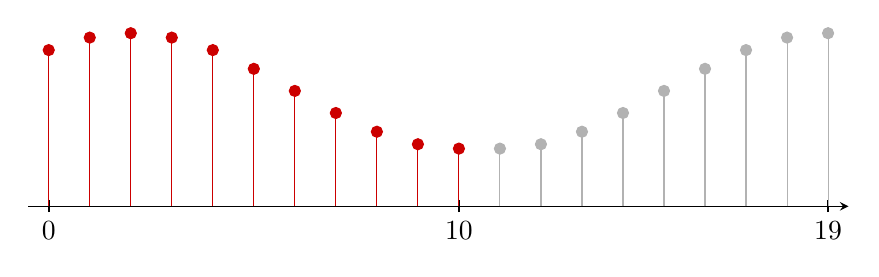
\begin{tikzpicture}
  \begin{axis}[
    width=12cm, height=4cm,
    axis x line=middle,
    axis y line=none,
    xmin=-0.5, xmax=19.5,
    ymin=0,
    xtick={0,10,19},
    xticklabels={0,10,19},              % keine Zahlen unterhalb
    ytick=\empty,
    tick style={black!50},
    major x tick style={black, thick},
    minor x tick style={black!20},
    minor x tick num=1,
  ]

    % rote Punkte (oben)
    \addplot+[ycomb, mark=*,
              draw=red!80!black,
              mark options={fill=red!80!black},
              every ycomb/.style={thin,red!80!black},
              every mark/.append style={draw=red!80!black}]
      coordinates {
        (0,4.061) (1,4.386) (2,4.5)   (3,4.386) (4,4.061)
        (5,3.574) (6,3)     (7,2.426) (8,1.939) (9,1.614)
        (10,1.5)
      };
    
    % graue Punkte (unten)
    \addplot+[ycomb, mark=*,
              draw=gray!60,
              mark options={fill=gray!60},
              every ycomb/.style={ultra thin,gray!60},
              every mark/.append style={draw=gray!60}]
      coordinates {
        (11,1.5)   (12,1.614) (13,1.939) (14,2.426)
        (15,3)     (16,3.574) (17,4.061) (18,4.386)
        (19,4.5)
      };
    

  \end{axis}
\end{tikzpicture}
\end{center}
\begin{center}
  \input{figures/dct2.tikz}
\end{center}
\begin{center}
  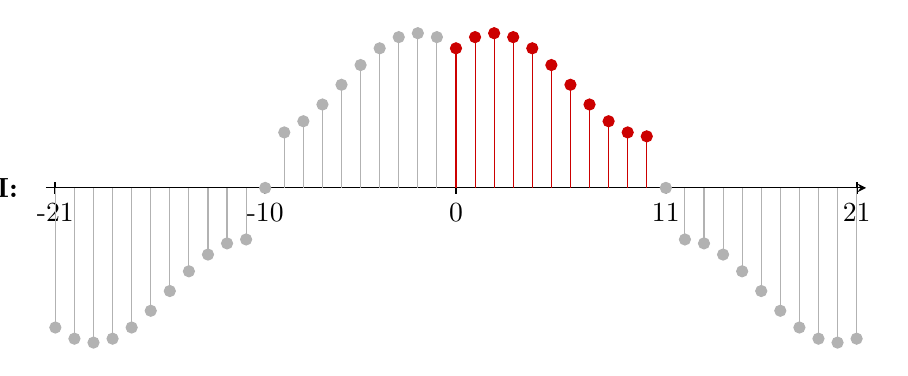
\begin{tikzpicture}
  \begin{axis}[
    width=12cm, height=6cm,
    axis x line=middle,
    axis y line=none,
    xmin=-21.5, xmax=21.5,
    ymin=-4.7,
    xtick={-21,-10, 0, 11,21},
    xticklabels={-21,-10, 0, 11,21},              % keine Zahlen unterhalb
    ytick=\empty,
    tick style={black!50},
    major x tick style={black, thick},
    minor x tick style={black!20},
    minor x tick num=1,
  ]
    % function used for the points: 3+1.5*cos(pi/8*(x-2))
    % red points
    \addplot+[ycomb, mark=*,
              draw=red!80!black,
              mark options={fill=red!80!black},
              every ycomb/.style={thin,red!80!black},
              every mark/.append style={draw=red!80!black}]
      coordinates {
        (0,4.061) (1,4.386) (2,4.5)   (3,4.386) (4,4.061)
        (5,3.574) (6,3)     (7,2.426) (8,1.939) (9,1.614)
        (10,1.5)
      };
    
    % gray points
    \addplot+[ycomb, mark=*,
              draw=gray!60,
              mark options={fill=gray!60},
              every ycomb/.style={ultra thin,gray!60},
              every mark/.append style={draw=gray!60}]
      coordinates {
        (11,0)
        (12, -1.5)  (13,-1.614) (14,-1.939) (15,-2.426)
        (16,-3)     (17,-3.574) (18,-4.061) (19,-4.386)
        (20,-4.5)   (21,-4.386) 
        (-1,4.386) (-2,4.5)   (-3,4.386) (-4,4.061)
        (-5,3.574) (-6,3)     (-7,2.426) (-8,1.939) (-9,1.614)
        (-10,0)
        (-11, -1.5)  (-12,-1.614) (-13,-1.939) (-14,-2.426)
        (-15,-3)     (-16,-3.574) (-17,-4.061) (-18,-4.386)
        (-19,-4.5)   (-20,-4.386) (-21, -4.061)
      };
    

  \end{axis}
  \node[anchor=east, xshift=0mm, overlay, font=\bfseries]
        at (current bounding box.west) {DCT-III:};
\end{tikzpicture}
\end{center}
\begin{center}
  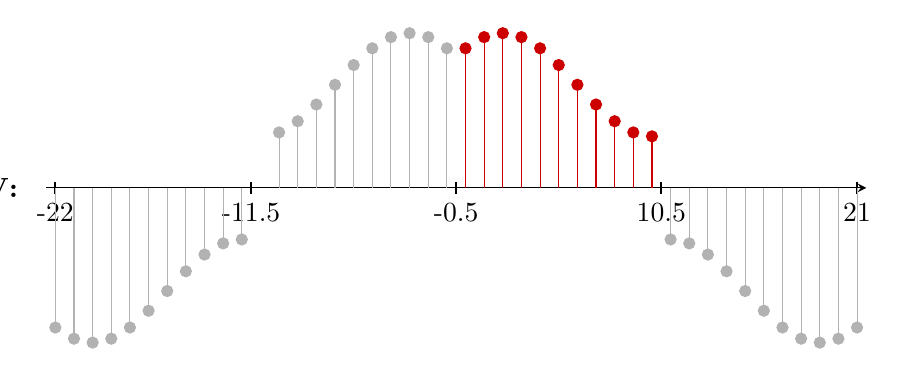
\begin{tikzpicture}
  \begin{axis}[
    width=12cm, height=6cm,
    axis x line=middle,
    axis y line=none,
    xmin=-22.5, xmax=21.5,
    ymin=-4.7,
    xtick={-22,-11.5, -0.5, 10.5,21},
    xticklabels={-22,-11.5, -0.5, 10.5,21},    
    ytick=\empty,
    tick style={black!50},
    major x tick style={black, thick},
    minor x tick style={black!20},
    minor x tick num=1,
  ]
    % function used for the points: 3+1.5*cos(pi/8*(x-2))
    % red points
    \addplot+[ycomb, mark=*,
              draw=red!80!black,
              mark options={fill=red!80!black},
              every ycomb/.style={thin,red!80!black},
              every mark/.append style={draw=red!80!black}]
      coordinates {
        (0,4.061) (1,4.386) (2,4.5)   (3,4.386) (4,4.061)
        (5,3.574) (6,3)     (7,2.426) (8,1.939) (9,1.614)
        (10,1.5)
      };
    
    % gray points
    \addplot+[ycomb, mark=*,
              draw=gray!60,
              mark options={fill=gray!60},
              every ycomb/.style={ultra thin,gray!60},
              every mark/.append style={draw=gray!60}]
      coordinates {
        (11, -1.5)  (12,-1.614) (13,-1.939) (14,-2.426)
        (15,-3)     (16,-3.574) (17,-4.061) (18,-4.386)
        (19,-4.5)   (20,-4.386) (21, -4.061)
        (-1,4.061) (-2,4.386) (-3,4.5)   (-4,4.386) (-5,4.061)
        (-6,3.574) (-7,3)     (-8,2.426) (-9,1.939) (-10,1.614)
        (-12, -1.5)  (-13,-1.614) (-14,-1.939) (-15,-2.426)
        (-16,-3)     (-17,-3.574) (-18,-4.061) (-19,-4.386)
        (-20,-4.5)   (-21,-4.386) (-22, -4.061)
      };
    

  \end{axis}
  \node[anchor=east, xshift=0mm, overlay, font=\bfseries]
        at (current bounding box.west) {DCT-IV:};
\end{tikzpicture}
\end{center}

\begin{colbox}{Satz}
  Die DCT-III und DCT-II Verfahren sind (bis auf Skalierung) invers zu einander. DCT-I und DCT-IV sind hingegen 
  selbst-invers.
\end{colbox}
\textit{ohne Beweis.}

\subsection{Mehrdimensionale DCT}
In der Anwendung dient DCT-II für die digitale Bildverarbeitung, wir müssen dafür jedoch eine Möglichkeit der 
mehrdimensionalen DCT finden. Wir nutzen hierfür die Spalten- bzw. Zeilenweise Anwendung von DCT-II und 
erhalten dann für $x\in\R^{N_1\times N_2}$ folgende Transformation
\begin{align*}
  \hat{x}_{k_1,k_2}
  = \sum_{n_1=0}^{N_1-1} \sum_{n_2=0}^{N_2-1}
  x_{n_1,n_2}
  \cos\Big(\dfrac{\pi}{N_1}\big(n_1+\tfrac{1}{2}\big)k_1\Big)
  \cos\Big(\dfrac{\pi}{N_2}\big(n_2+\tfrac{1}{2}\big)k_2\Big)
\end{align*}

Die mehrdimensionalen DCT ermöglicht uns nun eine Art der Bildkompression auf welcher auch die
JPEG-Kompression basiert. Als Vereinfachung betrachten wir lediglich die Kompression von Graustufenbildern, 
bei Farbbildern kann für jeden Farbkanal, z.B. rot,grün,blau, eine separierte Kompression
durchgeführt werden. Außerdem nehmen wir an, dass sich unser Bild in gleichgroße Quadrate zerlegend
lässt.

Die Grundidee besteht darin das Bild die Quadrate gleicher Größe zu zerlegen und diese einzeln zu
komprimieren, für JPEG üblich ist dabei die Wahl von $8\times 8$ Quadraten.

Gegeben eines Quadratausschnittes $x\in[0,1]^{N\times N}$ können wir nun die DCT durch
%
\begin{align*}
  \hat{x} = \sum_{n_1=0}^{N-1}\sum_{n_2=0}^{N-1} x\cdot b_{n_1,n_2}
\end{align*}
%
bestimmen, wobei
%
\begin{align*}
  b_{n_1,n_2} = \left(\cos\Big(\dfrac{\pi}{N_1}\big(n_1+\tfrac{1}{2}\big)k_1\Big)
  \cos\Big(\dfrac{\pi}{N_2}\big(n_2+\tfrac{1}{2}\big)k_2\Big)\right)_{k_1,k_2=0}^{N-1}
\end{align*}
%
die DCT-Basismatrizen beschreibt. Für größer werdendes N ergeben sich größere Feinheiten in der
Basis:

\begin{figure}[htbp]
  \centering
  \begin{minipage}{0.48\textwidth}
    \centering
    \includegraphics[width=\linewidth]{figures/dct_basis_grid_8.png}\\[2mm]
    \small $8 \times 8$ Basis
  \end{minipage}\hfill
  \begin{minipage}{0.48\textwidth}
    \centering
    \includegraphics[width=\linewidth]{figures/dct_basis_grid_16.png}\\[2mm]
    \small $16 \times 16$ Basis
  \end{minipage}
\end{figure}

Wenn wir auf unsere Transformierte $\hat{x}$ nun die mehrdimensionale DCT-III anwenden, so sollte wieder
unser ursprüngliches Bild herauskommen. Um eine Kompression zu erreichen speichern wir dann
nicht alle Komponenten unserer Transformierten, sondern nur einen Teil, indem zum Beispiel die
bestragskleinsten 90\% der Werte von $\hat{x}$ auf 0 setzten und so nur die größten 10\% behalten.

\subsection{Wavelets}
Bisher haben wir uns primär mit der Fourier-Transformation und ihren diskreten Varianten (DFT oder DCT) beschäftigt 
und diese als Werkzeug der Spektralanalyse kennengelernt. 

Die dafür verwendeten trigonometrischen Polynome ermöglichen eine einfache Trennung von nieder- und hochfrequenten 
Anteilen unseres Signals und verwenden dabei glatte Basisfunktionen. 

Ein wesentlicher Nachteil der Verwendung von Sinusoiden als Basis liegt in der Eigenschaft der globalen Ausdehnung, 
also dass jede Basisfunktion über dem gesamten Definitionsbereich \glqq{relevant}\grqq{} ist. Ohne einer 
lokalen Begrenzung gehen dadurch örtliche Informationen verloren. 

Außerdem kommt es bei der Annäherung von unstetigen Funktionen durch eine Fourier-Reihe zu
Über- und Unterschwingern an den Unstetigkeitsstellen, welche auch bei hohem Approximationsgrad
bestehen bleibt: \\

\begin{center}
  \includegraphics{figures/gibbsSquareWave100.png} \\
  \small Approximation eines Rechtecksignals mit Approximationsgrad 100
\end{center}

Um diesen Nachteilen entgegen zu wirken führen wir nun das Konzept der Wavelets als eine multiskalare Basis ein. 
Sie erlaubt ähnlich wie die Fourier-Analyse auch eine Frequenzzerlegung gewährleistet gleichzeitig aber auch eine 
zeitliche Lokalisierung. 

Wir wollen uns im folgenden lediglich auf die diskrete Wavelet-Transformation konzentrieren und betrachten dabei 
das Intervall $[0,1]$ als Definitionsbereich, d.h. wir suchen eine alternative Möglichkeit eine auf $[0,1]$ integrierbare 
Funktion $f$ approximieren. 

Wir beginnen damit absteigende Aufteilung des Intervall $[0,1]$ in äquidistante Teilintervalle zu definieren, 
für welche wir dann stückweise konstante Funktionen betrachten. 

\begin{colbox}{Definition}
  Sei $p\in\N$ fest. Für $k=0,1,\dots,p$ ist 
  %
  \begin{align*}
    \Delta_k := \{j\cdot h_k \,|\, j=0,\dots,2^k, k_k=2^{-k}\} \subset [0,1]
  \end{align*}
  %
  ein Gitter von Feinheitsgrad $k$. Die Unterteilung $\Delta_{k+1}$ entsteht dabei durch eine Verfeinerung 
  von $\Delta_k$. 

  Das feinste Gitter ist $\Delta_p$ mit Gitterweite $h_p=2^{-p}$ und das gröbste ist $\Delta_0$ mit Gitterweite $h_0=0$.

  Eine Skala von Funktionsräumen ergibt sich durch 
  %
  \begin{align*}
    V_0 \subset V_1 \subset \dots V_p
  \end{align*}
  %
  wobei $V_k$ der Raum aller Treppenfunktionen über $\Delta_k$ ist, d.h. 
  %
  \begin{align*}
    V_k := \{f:[0,1]\to\R \,|\, \forall j=0,\dots,2^k-1: f \text{ konstant auf } I_{k,j}=[j\cdot h_k, (j+1)\cdot h_k] \}
  \end{align*}
  %
\end{colbox}

Eine triviale Basis von $V_k$ bilden dabei die charakteristischen Funktionen auf $I_{k,j}$ und eine Skalierung 
mit $2^{k/2}$ macht diese Basis zu einem Orthonormalsystem:

\begin{colbox}{Satz}\label{satz:chiOrthonorm}
  Die Menge $\{\chi_{k,j}\}_{j=0}^{2^k-1}$ mit $\chi = \chi_{[0,1]}$ und
  %
  \begin{align*}
    \chi_{k,j}(x) = 2^{k/2}\chi(2^kx-j) = \begin{cases}
      2^{k/2}, &x\in I_{k,j}\\
      0, &\text{sonst}
    \end{cases} 
  \end{align*}
  %
  bildet eine Orthonormalbasis von $V_k$ bzgl. dem $L^2$-Skalarprodukt.
\end{colbox}
\textit{Beweis.}
\begin{enumerate}
  \item Jede Funktion $f\in V_k$ lässt sich nach Definition von $V_k$ als Treppenfunktionen über $\Delta_k$ schreiben, 
  d.h. sie hat die Darstellung 
  \begin{align*}
    f(x) 
    = \sum_{j=0}^{2^k-1} c_j\cdot \chi_{I_{j,k}}(x)
    = \sum_{j=0}^{2^k-1} 2^{-k/2}c_j\cdot \chi_{j,k}(x) \in 
    \Span\{\chi_{k,j} \,|\, j=0,\dots,2^k-1\}
  \end{align*}
  \item Für $j\neq l$ ist $I_{j,k}\cap I_{l,k}$ endlich und es gilt:
  \begin{align*}
    &\int_{0}^{1} \chi_{j,k}(x) \cdot \chi_{l,k}(x) \diff x \\
    &\quad = 2^{k}\cdot \int_{0}^{1} \chi_{I_{j,k}}(x) \cdot \chi_{I_{l,k}}(x) \diff x \\
    &\quad = 2^{k}\cdot\left(
      \int_{I_{j,k}} \underbrace{\chi_{I_{j,k}}(x)}_{1} \cdot \underbrace{\chi_{I_{l,k}}(x)}_{0} \diff x
      + \int_{I_{j,k}} \underbrace{\chi_{I_{j,k}}(x)}_{0} \cdot \underbrace{\chi_{I_{l,k}}(x)}_{1} \diff x
      + \int_{[0,1]\backslash(I_{j,k}\cup I_{l,j})} 
      \underbrace{\chi_{I_{j,k}}(x)}_{0} \cdot \underbrace{\chi_{I_{l,k}}(x)}_{0}  \diff x
    \right) \\
    &\quad = 2^{k} \left(\Big((j+1)2^{-k} - j2^{-k}\Big) + \Big((l+1)2^{-k} - l2^{-k}\Big) + 0\right) \\
    &\quad = 0
  \end{align*}
  Im Fall $l=j$ ergibt sich:
  \begin{align*}
    \int_{0}^{1} \underbrace{\chi_{j,k}(x)^2}_{0^2=0, 1^2=1} \diff x 
    = 2^k \cdot \int_{0}^{1} \chi_{I_{j,k}}(x) \diff x 
    = 2^k \cdot \Big((j+1)2^{-k} - j2^{-k}\Big) 
    = 1
  \end{align*}
  Damit bildet die Menge ein Orthonormalsystem, also auch linear unabhängig ist durch 1. eine Orthonormalbasis.
  \qed
\end{enumerate}

\begin{colbox}{Bemerkung}
  Es gilt $\chi(x) = \chi(2x) + \chi(2x-1)$ und damit folgt
  %
  \begin{align*}
    \chi_{k,j} 
    = \dfrac{1}{\sqrt{2}}\Big(\chi_{k+1,2j}(x) + \chi_{k+1,2j+1}(x)\Big)
  \end{align*}
  %
\end{colbox}

Die Idee hinter Wavelets ist es nun für eine Festes $k$ das Gitter $\Delta_k$ zu $\Delta_{k+1}$ zu verfeinern. 
Da wir wissen, dass $V_k$ ein Unterraum von $V_{k+1}$ ist, 
lässt sich die Basis $\{\chi_{k,j}\}_{j=0}^{2^k-1}$ zu einer Basis 
von $V_{k+1}$ erweitern. Durch die Setzung $W_k = V_{k+1} \cap V_k^\perp$ ergibt sich 
%
\begin{align*}
  V_{k+1} = V_k \oplus W_k
\end{align*}
%
und wir können durch das finden einer Basis von $W_k$ eine Basis von $V_k$ konstruieren. Für die Basis 
$\{\psi_{k,j}\}_{j=0}^{2^k-1}$ fordern wir erneut die Schreibweise in Abhängigkeit einer Grundfunktion $\psi$:
%
\begin{align*}
  \psi_{k,j}(x) = 2^{k/2}\psi(2^kx-j) 
  \tag{1} \label{eq:waveletsEQ1}
\end{align*}
%
sowie die Bedingung $\psi_{k,j}\in W_k$, d.h. 
%
\begin{align*}
  \psi_{k,j} &\in V_{k+1} 
  \tag{2}\label{eq:waveletsEQ2}\\
  \langle\psi(k,j), \chi_{k,l}\rangle_2 &= 0 \qquad \text{für alle } l=0,\dots,2^k-1
  \tag{3}\label{eq:waveletsEQ3}
\end{align*}
%
Außerdem wollen wir auch hier wieder eine Orthonormalbasis, also fordern wir weiter 
%
\begin{align*}
  \langle\psi(k,j), \psi_{k,l}\rangle_2 &= \delta_{jl} = \begin{cases}
    1, \quad & j=l \\
    0, \quad & j\neq l
  \end{cases} \qquad \text{für alle } l=0,\dots,2^k-1
  \tag{4}\label{eq:waveletsEQ4}
\end{align*}
%
\begin{colbox}{Lemma}
  Für die Funktion
  %
  \begin{align*}
    \psi(x) := \chi(2x) - \chi(2x-1) = \begin{cases}
      1, \quad & 0\leq x\leq \tfrac{1}{2}\\
      -1, \quad & \tfrac{1}{2}\leq x\leq 1 \\
      0, \quad & \text{sonst}
    \end{cases}
  \end{align*}
  %
  erfüllen $\{\psi_{k,j}\}_{j=0}^{2^k-1}$ aus (\ref{eq:waveletsEQ1}) die 
  Bedingungen (\ref{eq:waveletsEQ2}), (\ref{eq:waveletsEQ3}) und (\ref{eq:waveletsEQ4}).
\end{colbox}

\textit{Beweis.} 
\begin{enumerate}
  \item[(2)] 
  Für $j=0,\dots,2^k-1$ gilt 
  \begin{align*}
    \psi_{k,j} 
    = 2^{k/2}\psi(2^kx-j) 
    &= 2^{k/2}\Big(\chi(2^{k+1}x-j)-\chi(2^{k+1}x-2j-1)\Big) \\
    &= \dfrac{1}{\sqrt{2}}\Big(\chi_{k+1,2j}(x) - \chi_{k+1,2j+1}(x)\Big)
    %\tag{5}(\label{eq:waveletsEQ5})
  \end{align*}
  %
  Da wir wissen, dass $\{\chi_{k+1,j}\}_{j=0}^{2^{k+1}-1}$ eine Basis von $V_{k+1}$ ist, folgt $\psi_{k,j}\in V_{k+1}$.
  \item[(3)] Verwenden wir die Darstellungen von $\psi_{k,j}$ und $\chi_{k,j}$ durch $\{\chi_{k+1,j}\}_{j=0}^{2^{k+1}-1}$
  erhalten wir durch Satz \ref{satz:chiOrthonorm} die geforderte Orthogonalität für $j\neq k$:
  %
  \begin{align*}
    \langle \psi_{k,j}, \chi_{k,l} \rangle
    &= \left\langle \dfrac{1}{\sqrt{2}}\Big(\chi_{k+1,2j}(x) - \chi_{k+1,2j+1}(x)\Big), 
    \dfrac{1}{\sqrt{2}}\Big(\chi_{k+1,2l}(x) + \chi_{k+1,2l+1}(x)\Big) \right\rangle _2 \\
    &= \dfrac{1}{2}\left(
      \underbrace{\langle \chi_{k+1,2j}(x), \chi_{k+1,2l}(x) \rangle_2}_{0}
      + \underbrace{\langle \chi_{k+1,2j}(x), \chi_{k+1,2l+1}(x) \rangle_2}_{0}\right.\\
      &\qquad \left.- \underbrace{\langle \chi_{k+1,2j+1}(x), \chi_{k+1,2l}(x) \rangle_2}_{0}
      - \underbrace{\langle \chi_{k+1,2j+1}(x), \chi_{k+1,2l+1}(x) \rangle_2}_{0} 
    \right)\\
    &= 0
  \end{align*}
  %
  \item[(4)] Analog erhalten wir auch, dass $\{\psi_{k,j}\}_{j=0}^{2^k-1}$ ein Orthonormalsystem bildet.
\end{enumerate}

\begin{colbox}{Bemerkung}
  Im allgemeinen werden die Funktion $\chi$ und $\psi$ Vater- und Mutter-Wavelet genannt. Für unseren speziellen Fall 
  heißt $\{\psi_{k,j}\}_{j=0}^{2^k-1}$ Haar-Wavelet-Basis. 

  Neben der Haar-Wavelet-Basis ergeben sich durch andere Wahlen von $\chi$ und $\psi$ neue Basismengen, Beispiele 
  hierfür sind Meyer-Wavelet, Mexikanischer Hut oder Daubechies D4-Wavelet:

  \begin{minipage}[t]{.49\textwidth}
    \includegraphics[width=\linewidth]{figures/haar_wavelet.png}\\[4pt]
    \includegraphics[width=\linewidth]{figures/mexican_hat_wavelet.png}
  \end{minipage}\hfill
  \begin{minipage}[t]{.49\textwidth}
    \includegraphics[width=\linewidth]{figures/daubechies_d4_wavelet.png}\\[4pt]
    \includegraphics[width=\linewidth]{figures/meyer_wavelet.png}
  \end{minipage}
\end{colbox}

Das Finden einer Basis für $W_{k}$ erlaubt das konstruieren einer neuen Basis von $V_{k+1}$, diese nennen wir 
auch Zweiskalenbasis. Durch das rekursive Zerlegen von $V_k=V_{k-1}+W_{k-1}$ erhalten wir 
%
\begin{align*}
  V_p = V_0 \oplus W_0 \oplus W_1 \oplus \dots \oplus W_{p-1}
\end{align*}
%
mit der Basis 
%
\begin{align*}
  \{\chi_{0,0}\}
  \cup \{\psi_{1,0}, \psi_{1,1}\}
  \cup \{\psi_{2,0},\dots,\psi_{2,3}\} 
  \cup \dots \cup\{\psi_{p-1,0}, \dots, \psi_{p-1,2^{p-1}-1}\}
\end{align*}
%
wobei $\chi_{0,0}$ auf $[0,1]$ einfach nur konstant $1$ ist.

\begin{colbox}{Bemerkung}
  Wie auch schon bei der Fourier-Transformation sind wir nun in der Lage eine Bestapproximation zu $f$ im Raum $V_k$ 
  zu finden, die Wavelet-Transformation. Auch hier lässt sich daraus eine diskrete Wavelet-Transformation und eine 
  schnelle Wavelet-Transformation herleiten. 
\end{colbox}